
\documentclass[runningheads]{llncs}
\usepackage[text={150mm,220mm},centering]{geometry}
\usepackage{graphicx}
\usepackage{hyperref}
\usepackage{color}
\hypersetup{
    colorlinks=true,
    linkcolor=blue,
    filecolor=blue,      
    urlcolor=blue,
    citecolor=cyan,
}

\begin{document}
\title{\large{CSCI927 Service-Oriented Software Engineering (Assignment)}}
%--------------------Please do NOT change the content above.-------------------------------------------------

%
%----Please write your personal information as below.------------------------------------
%
\author{\large{Student Name: Xiao Yao \\ % Please write your name here
CCNU Student Number: 2019180015 \\ % Please write your CCNU student number here
UOW Student Number: 6641751}}  % Please write your UOW student number here


%-----------------------------------------------------------------------------------------------



%---------Do not change the content of this part--------------------

\authorrunning{CCNU Wollongong Joint Institute}
\institute{Central China Normal University Wollongong Joint Institute}

\maketitle


%-----------Please write your solutions to the questions in the assignment from here.---------------

\section{PART ONE (7 MARKS)}
\subsection{Description on Designed Insurance Claim Handling Process}
%-----------------------------------------------------------------------------------------------------------------------
% In this subsection, you need to describe your designed insurance claim handling process in your own words. You also need to provide the sources from which you developed the process model, e.g., a link where the sources are from, a published paper's name from which conference/journal/workshop, etc.
%----------------------------------------------------------------------------------------------------------------------%
Considering that the insurance claim process is not a single act, but an interactive act, I chose to use lanes to represent different roles, including customers and bank assessors. At the same time, insurance claims are also a complicated and task-intensive process. In order to better understand the situation of each customer, you first need to fill out a detailed application form. If the application form is not completed, a rejection letter will be sent. After the application form is completed, check whether the customer is eligible for insurance according to the content filled out by the customer. If the qualification is not qualified, a rejection letter will be sent. If the qualification is met, the next stage will be entered to calculate the insurance amount. However, if it is impossible to judge the need to re-examine, it is necessary. Transfer it to the bank assessor for review. If the bank assessor is still unable to judge, the exception is thrown directly, and a rejection letter is sent. If the bank assessor checks both the condition and all the information, the application is agreed and the insurance amount is calculated. After calculating according to the payment conditions, the insurance policy is sent to the user for confirmation. After receiving the confirmation email, the user needs to wait for one working day to receive the payment and the payment documents.\\ Here is my references:
\begin{enumerate}
    \item \url{https://www.signavio.com/post/insurance-example-processing-a-claim/ }
    \item \url{https://consumer.findlaw.com/insurance/the-insurance-claim-process.html}
    \item \url{https://www.oecd.org/finance/insurance/33964905.pdf}
    \item \url{https://www.dir.ca.gov/dwc/InjuredWorkerInfo/Claimsprocess.pdf}
\end{enumerate}



\subsection{Designed BPMN Model}
%-----------------------------------------------------------------------------------------------------------------------
% Please insert your designed BPMN model as a figure in this subsection.
% Please note that your designed BPMN must match with the description that you have summarized in the previous subsection.
%----------------------------------------------------------------------------------------------------------------------%
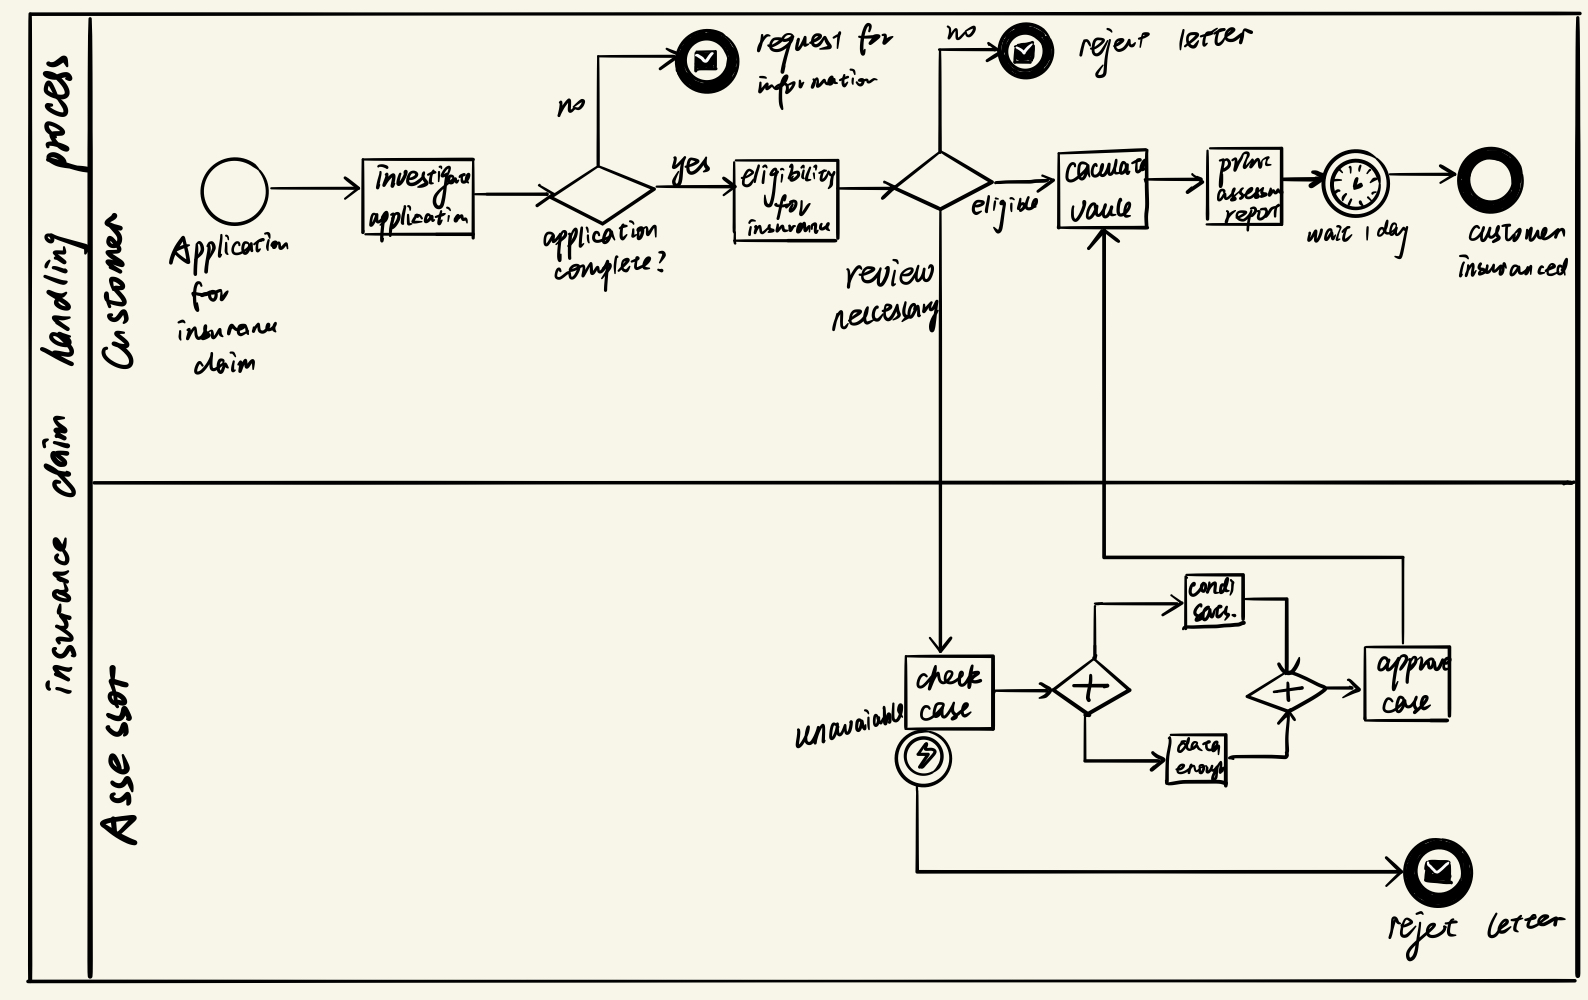
\includegraphics[scale=0.3]{BPMN.jpeg}






\subsection{Semantic Effect Annotation}
%-----------------------------------------------------------------------------------------------------------------------
% Please insert your designed BPMN model with Text Annotations on your BPMN model as a figure in this subsection.
%----------------------------------------------------------------------------------------------------------------------%
\begin{enumerate}
    \item Objects of interests: Application a, Claim c, Outcome c, Amount t
    \item States:
        \begin{itemize}
            \item[·] Application rejected or approved - rejected(a), approved(a)
            \item[·] Claim rejected or approved or  eligible or reviewed - rejected(c), approved(c), eligible(c), reviewed(c)
        \end{itemize}
    \item Relationships between objects:
        \begin{itemize}
            \item[·] Application investigated with an outcome - investigated(a,o)
            \item[·] Claim eligibility with an outcome - eligibility(c,o)
            \item[·] Claim checked with an outcome - checked(c,o)
            \item[·] Claim satisfied with conditions - satisfied(c,n)
            \item[·] Claim examed with data - examed(c,d)
            \item[·] Claim calculated with an amount - calculated(c,t)
            \item[·] Claim assessed with a report - assessed(c,r)
        \end{itemize}
    
\end{enumerate}









\begin{itemize}
\item[(a)]{Cumulative Effects of Tasks/Activities}
%----------------------------------------------------------------------------------------------------------------------
% Please provide the cumulative effects of tasks/activities as required.
%----------------------------------------------------------------------------------------------------------------------%
\begin{enumerate}
    \item Reject Application: \textcolor{red}{investigated(a,o) $\land$ rejected(a)}
    \item Store Username: \textcolor{red}{investigated(a,o) $\land$ approved(a) $\land$ approved(u) $\land$ stored(u,s)}
    \item Reject Update Username: \textcolor{red}{investigated(a,o) $\land$ approved(a) $\land$ approved)(u) $\land$ interrupted(u) $\land$ rejected(u)}
    \item Update Username: \textcolor{red}{investigated(a,o) $\land$ approved(a) $\land$ approved(u) $\land$ stored(u,s) $\land$ updated(u,s)}
    \item Receive Status: \textcolor{red}{investigated(a,o) $\land$ approved(a) $\land$ approved(u) $\land$ stored(u,s) $\land$ updated(u,s) $\land$ received(u,s)}
    
\end{enumerate}



\newpage\item[(b)]{Cumulative Effect Scenarios}
%----------------------------------------------------------------------------------------------------------------------
% Please provide the cumulative effect scenarios obtained at various points in the process as required.
%----------------------------------------------------------------------------------------------------------------------%

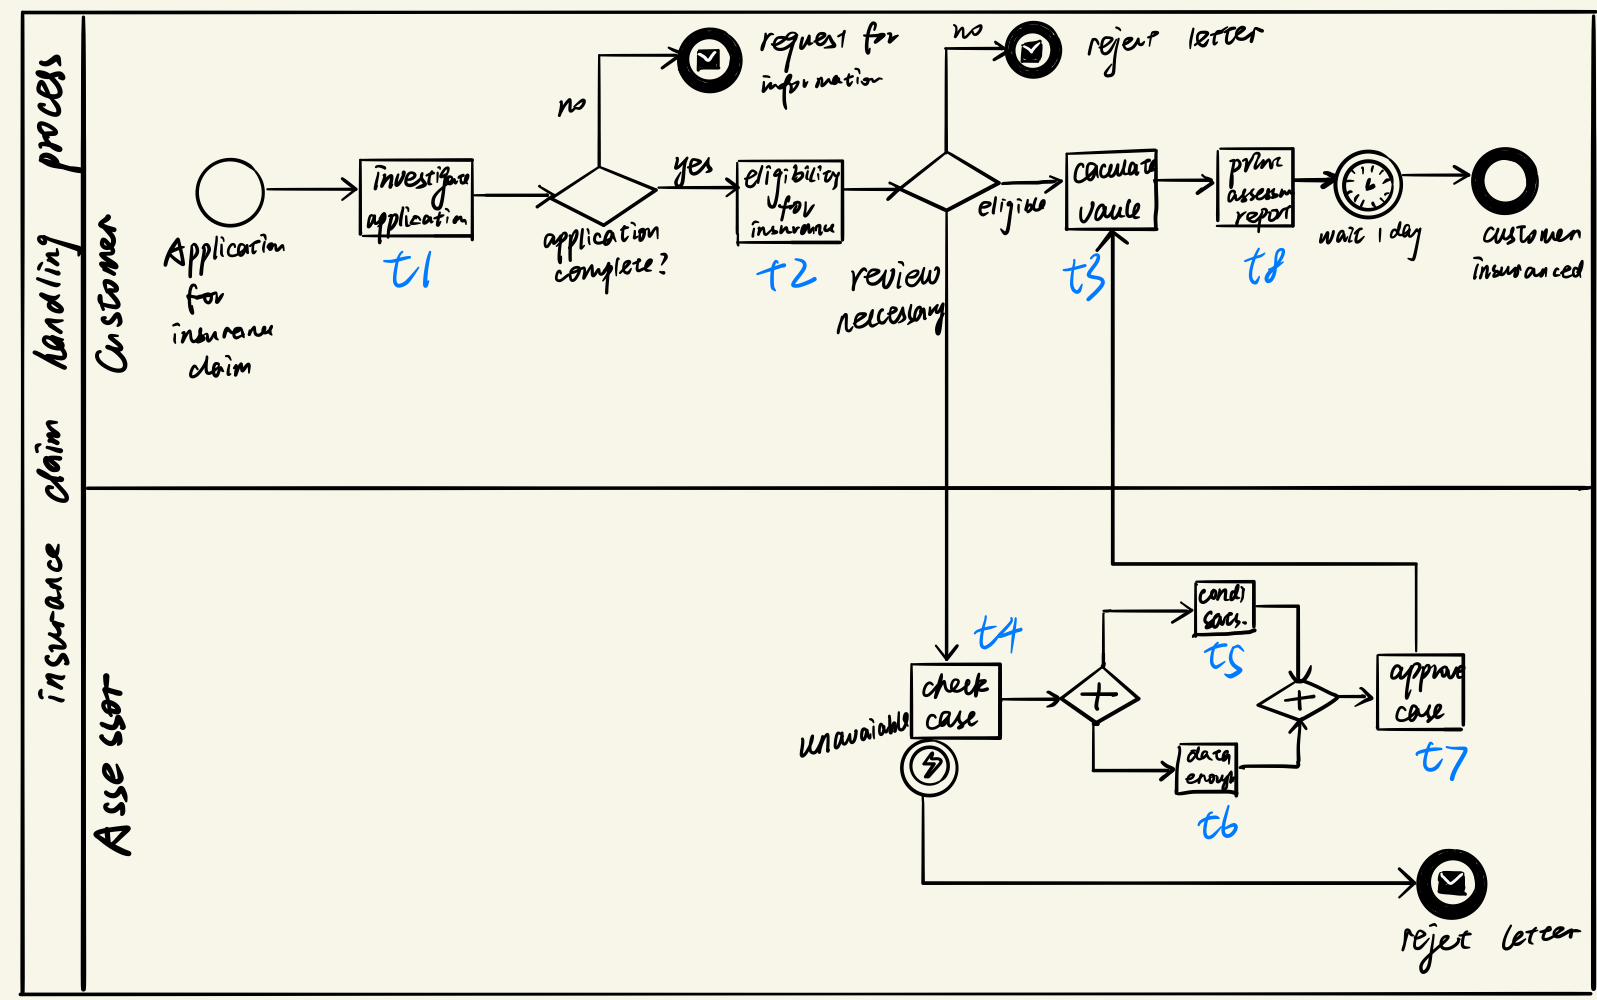
\includegraphics[scale=0.18]{scenario.jpeg}
\begin{enumerate}
    \item $t_3$:
        \begin{itemize}
            \item[·] Scenario(1): $\left \langle \langle t_1,t_2,\left\{\langle t_3 \rangle \right\} \rangle, \left\{\langle t_1,t_2,t_4,\left\{\langle t_5,t_6 \rangle \right\},t_7 \rangle \right\}\right \rangle$
            \item[·] Scenario(2): $\left \langle \langle t_1,t_2,t_4,\left\{\langle t_5,t_6 \rangle \right\},t_7,\left\{\langle t_3 \rangle \right\} \rangle, \left\{\langle t_1,t_2 \rangle\right\}\right \rangle$
        \end{itemize}
    \item $t_8$:
        \begin{itemize}
            \item[·] Scenario(1): $\left \langle \langle t_1,t_2,t_3,\left\{\langle t_8 \rangle \right\}\rangle, \left\{\langle t_1,t_2,t_4,\left\{\langle t_5,t_6 \rangle \right\},t_7,t_3 \rangle \right\}\right \rangle$
            \item[·] Scenario(2): $\left \langle \langle t_1,t_2,t_4,\left\{\langle t_5,t_6 \rangle \right\},t_7,t_3,\left\{\langle t_8 \rangle \right\}\rangle , \left\{\langle t_1,t_2,t_3 \rangle \right\}\right \rangle$
            
        \end{itemize}
    
\end{enumerate}





\end{itemize}

\section{PART TWO (3 MARKS)}
\subsection{Designed Petri Net}
%----------------------------------------------------------------------------------------------------------------------
% Please insert your designed Petri Net as a figure as required in this subsection.
%----------------------------------------------------------------------------------------------------------------------%
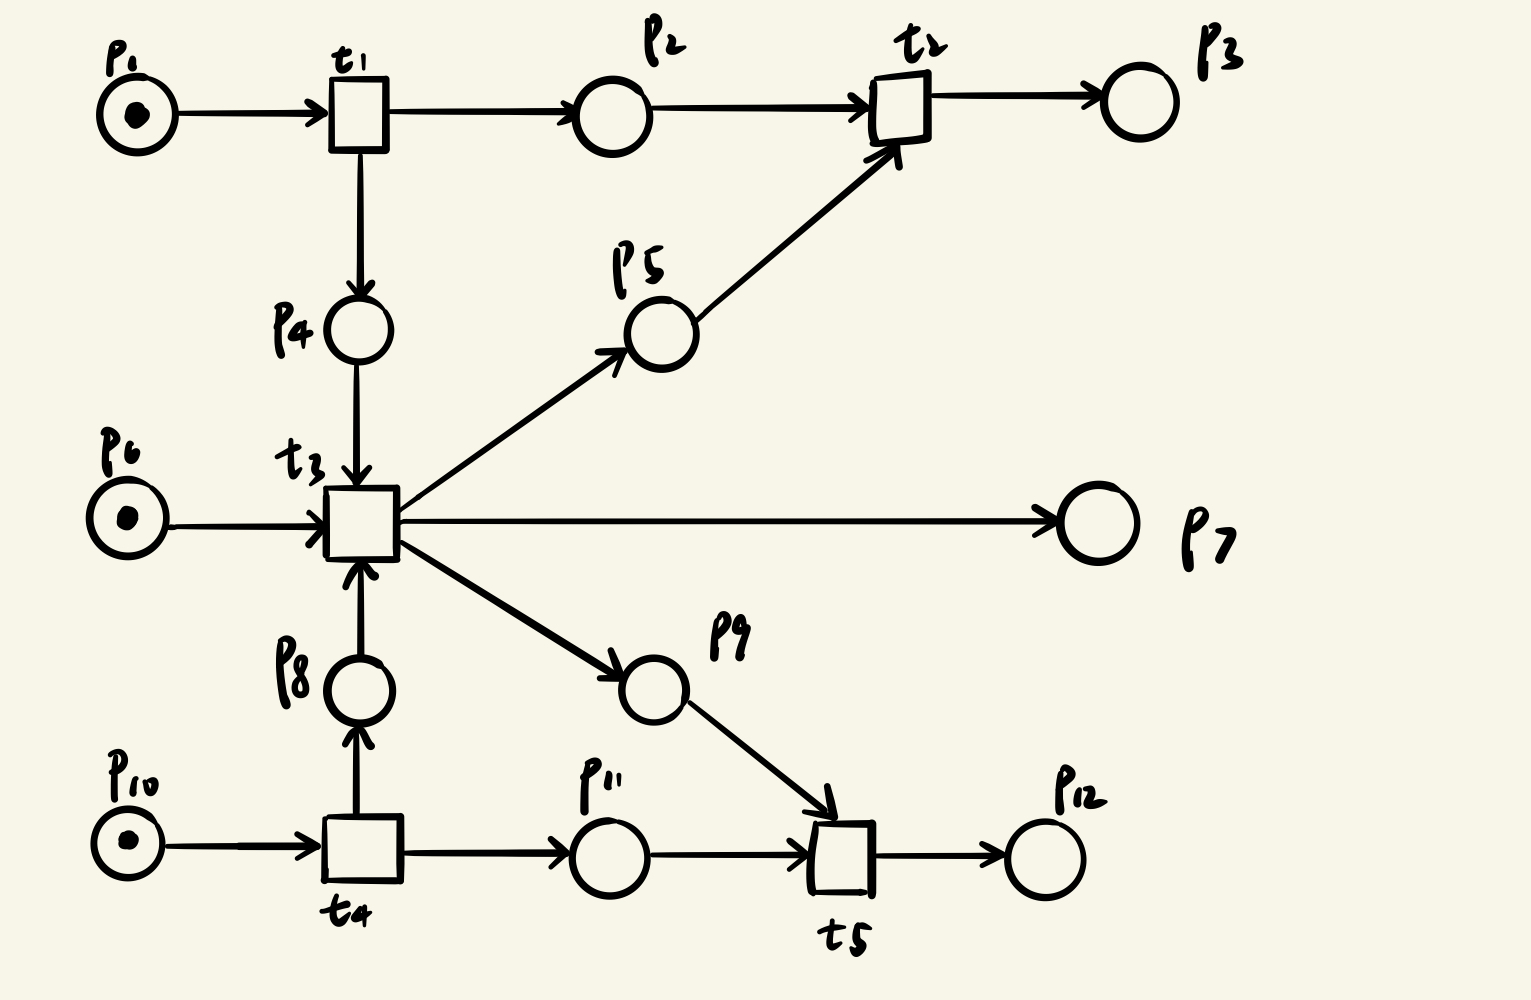
\includegraphics[scale=0.2]{car-racing.jpeg}


\subsection{Analysis on the Petri Net}
%----------------------------------------------------------------------------------------------------------------------
% Please give your analysis on your designed Petri Net by playing with a ``token game" in this subsection.
%----------------------------------------------------------------------------------------------------------------------%

% \begin{enumerate}
%     \item It can see that the t_1 conditions{p_1,p_2,p_4}, so the token start with the p_1 and p_10, and concurrent actions t_1 and t_4
% \end{enumerate}


\begin{enumerate}
    \item It can see that the $t_1$ conditions$\left\{p_1,p_2,p_4\right\}$, so the token start with the $p_1$ and $p_{10}$, and pass by concurrent actions $t_1$ and $t_4$.\\ 
    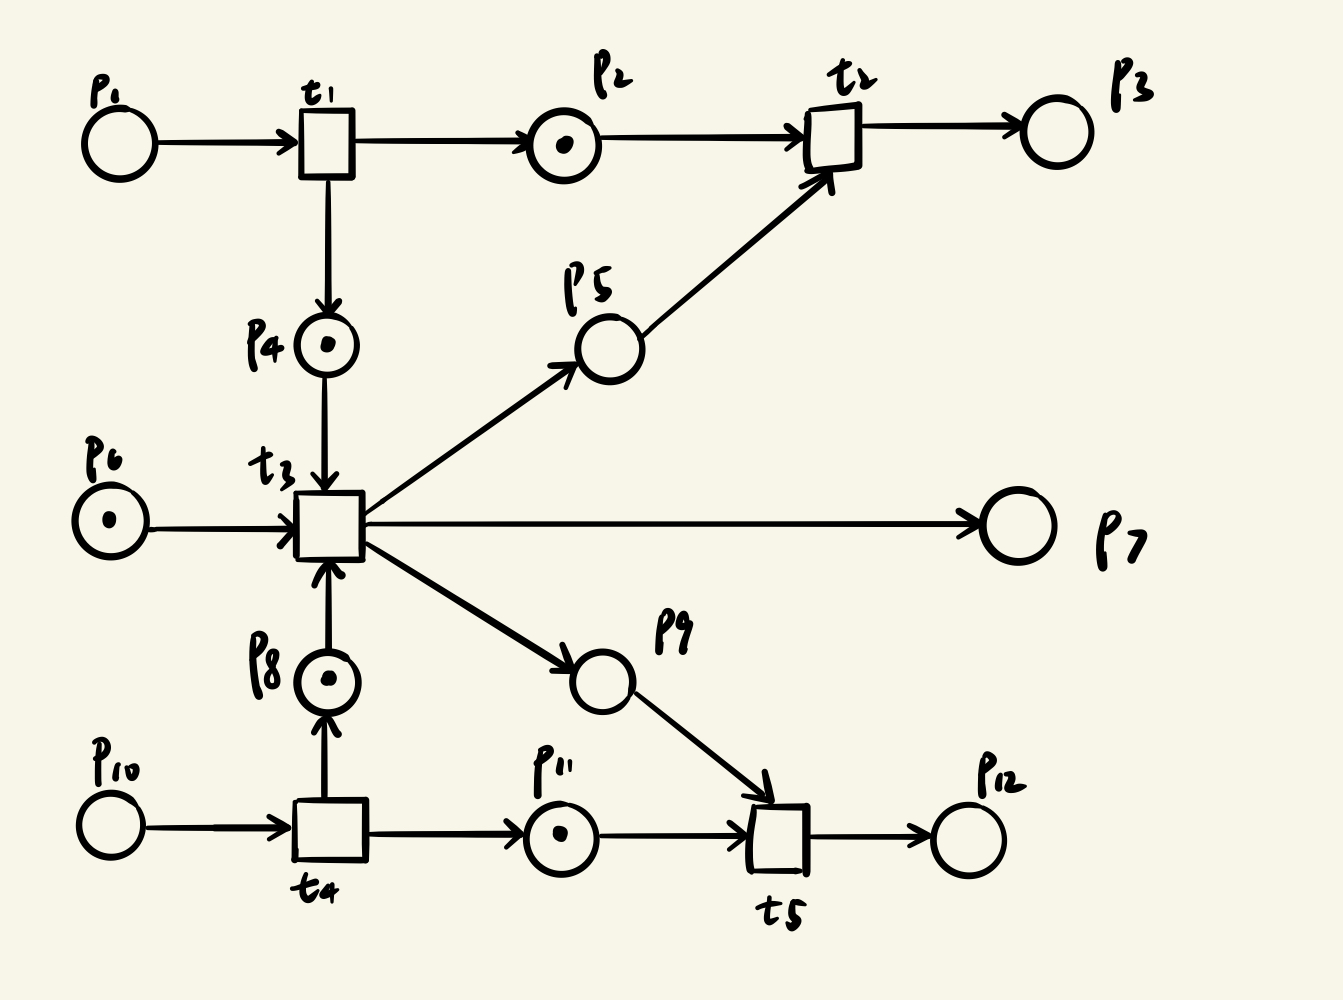
\includegraphics[scale=0.15]{token1.jpeg}
    \item And then input p of $t_3$ is marked with $w((p,t))$ tokens, so the transition $t_3$ is enabled, the token pass by $t_3$ to $p_7$.\\
    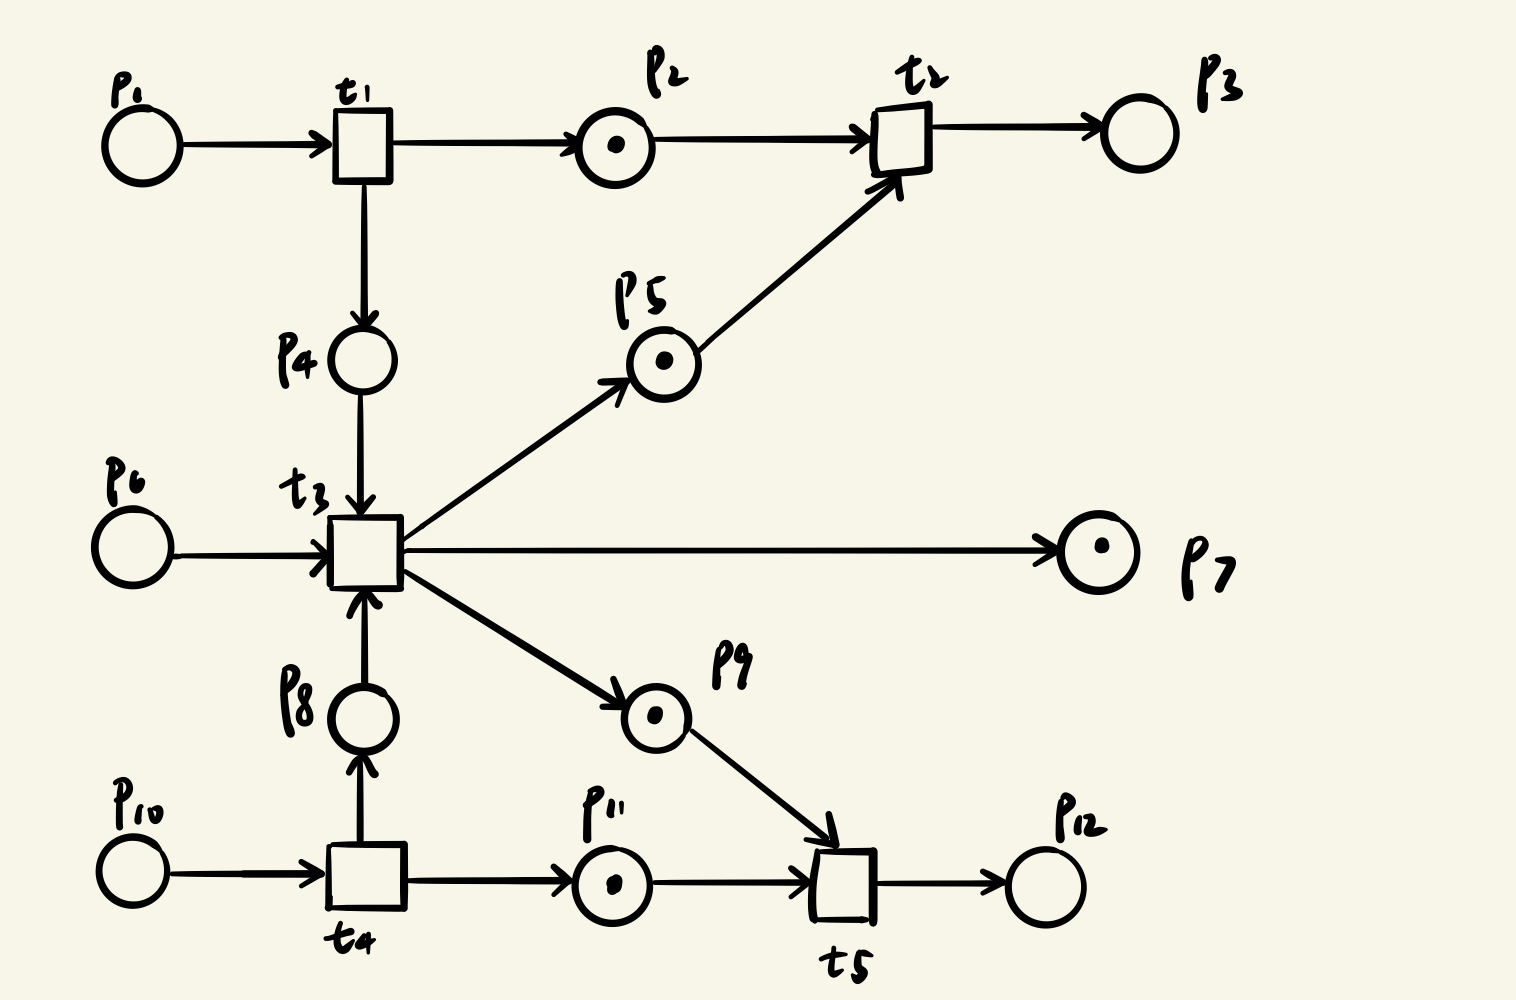
\includegraphics[scale=0.15]{token2.jpeg}
    \item At last, the same as above, transition $t_2$ and $t_5$ is enabled, the racing game is over.\\
    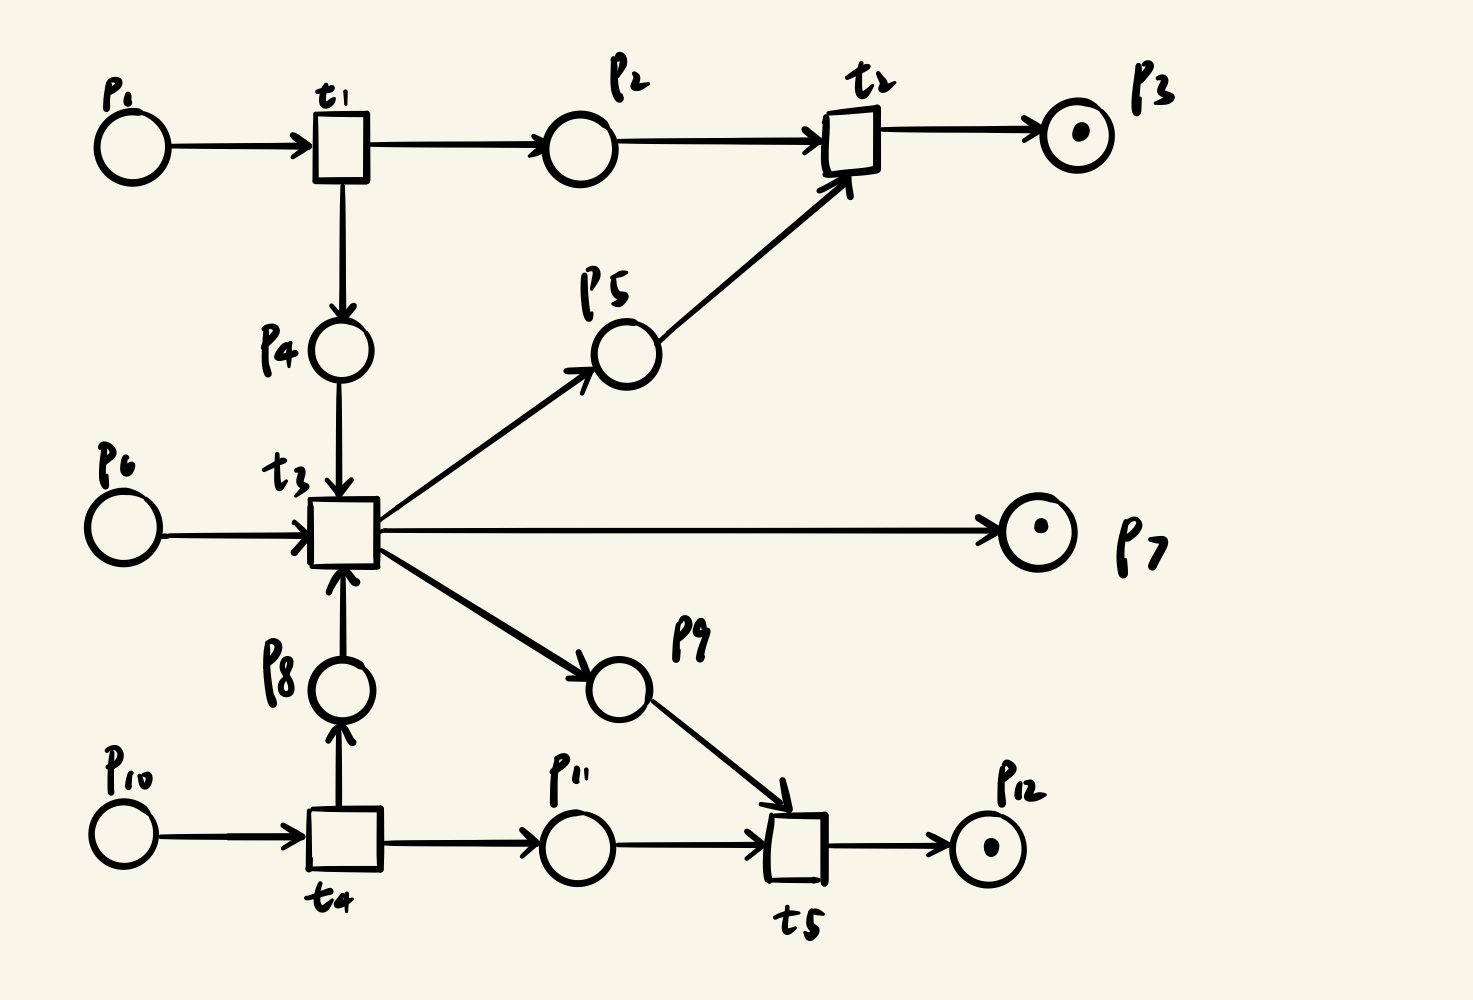
\includegraphics[scale=0.15]{token3.jpeg}
    
\end{enumerate}


\end{document}
